\documentclass{beamer}

% This file is a solution template for:

% - Giving a talk on some subject.
% - The talk is between 15min and 45min long.
% - Style is ornate.



% Copyright 2004 by Till Tantau <tantau@users.sourceforge.net>.
%
% In principle, this file can be redistributed and/or modified under
% the terms of the GNU Public License, version 2.
%
% However, this file is supposed to be a template to be modified
% for your own needs. For this reason, if you use this file as a
% template and not specifically distribute it as part of a another
% package/program, I grant the extra permission to freely copy and
% modify this file as you see fit and even to delete this copyright
% notice. 


\mode<presentation>
{
  \usetheme{Warsaw}
  % or ...

  \setbeamercovered{transparent}
  % or whatever (possibly just delete it)
}


\usepackage[english]{babel}
% or whatever

\usepackage[utf8]{inputenc}
% or whatever

\usepackage{times}
\usepackage[T1]{fontenc}
% Or whatever. Note that the encoding and the font should match. If T1
% does not look nice, try deleting the line with the fontenc.

\usepackage{pgfgantt}

\title[Restraint Selection in PSP] % (optional, use only with long paper titles)
{Improve the use of noisy restraints in ab initio protein structure prediction}

%\subtitle
%{Presentation Subtitle} % (optional)

\author%[Author, Another] % (optional, use only with lots of authors)
{David Lassner, Moritz Neeb}
% - Use the \inst{?} command only if the authors have different
%   affiliation.

\institute[Universities of Somewhere and Elsewhere] % (optional, but mostly needed)
{
  Computational Biology Project\\
  TU Berlin}
% - Use the \inst command only if there are several affiliations.
% - Keep it simple, no one is interested in your street address.

\date%[Short Occasion] % (optional)
{Dec 12, 2014}

\subject{Talks}
% This is only inserted into the PDF information catalog. Can be left
% out. 



% If you have a file called "university-logo-filename.xxx", where xxx
% is a graphic format that can be processed by latex or pdflatex,
% resp., then you can add a logo as follows:

% \pgfdeclareimage[height=0.5cm]{university-logo}{university-logo-filename}
% \logo{\pgfuseimage{university-logo}}



% Delete this, if you do not want the table of contents to pop up at
% the beginning of each subsection:
%\AtBeginSubsection[]
%{
%  \begin{frame}<beamer>{Outline}
%    \tableofcontents[currentsection,currentsubsection]
%  \end{frame}
%}


% If you wish to uncover everything in a step-wise fashion, uncomment
% the following command: 

%\beamerdefaultoverlayspecification{<+->}


\begin{document}

\begin{frame}
  \titlepage
\end{frame}

\begin{frame}{Outline}
  \tableofcontents
  % You might wish to add the option [pausesections]
\end{frame}

\section{Insights on constraints}
\begin{frame}{constraints}
%    \begin{columns}[c] % the "c" option specifies center vertical alignment
%    \column{.5\textwidth} % column designated by a command
    \centering
    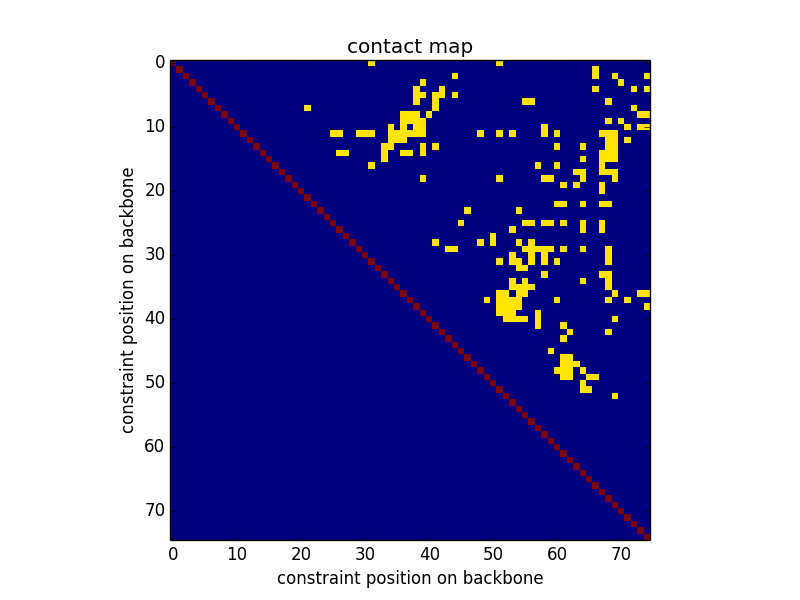
\includegraphics[width=0.7\textwidth]{img/contactMap}
%    \column{.5\textwidth} % column designated by a command
    \begin{itemize}
    \item There are some clusters
    \item There are no constraints for near-by position
    \end{itemize}
%    \end{columns}
\end{frame}


\begin{frame}{natives}
    \centering
    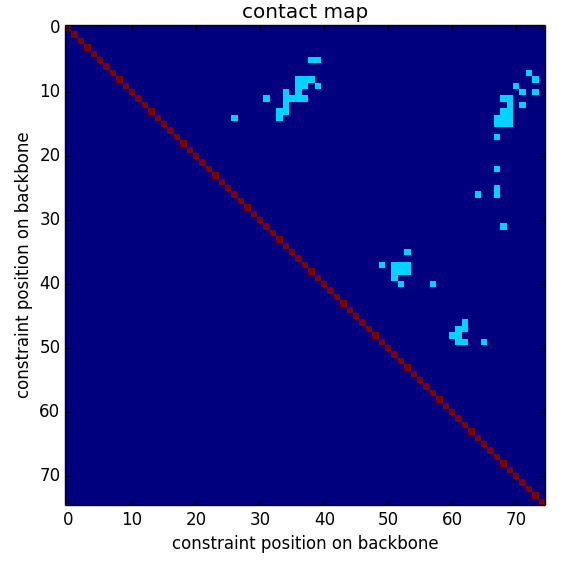
\includegraphics[width=0.5\textwidth]{img/contactMapNatives}
    \begin{itemize}
    \item Some positions have connections to a broad area of the sequence
    \end{itemize}
\end{frame}

\begin{frame}{Constraint visualisation}
    \centering
    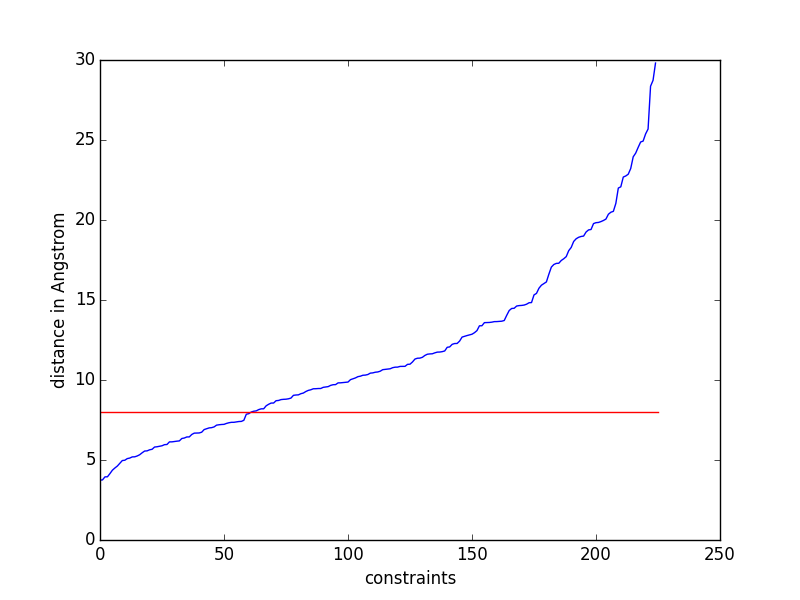
\includegraphics[width=0.7\textwidth]{img/constraintGroundTruth}
    \begin{itemize}
    \item Many constraints from the file are not activated in the native structure
    \end{itemize}
\end{frame}

%\begin{frame}{Contraint combinations}
%\begin{tabular}{lllll}
    %pos &1& pos &2& distance\\\hline
    %CB &9 &CB &37 &5.45\\
    %CB &9 &CB &38 &6.68\\
    %CB &9 &CB &39 &4.62\\\hline
    %%&\vspace{.5cm}&&&&\\
    %CB &10& CB& 37& 6.74\\
    %CB &10& CB& 38& 5.25\\
    %CB &10& CB& 39& 8.15\\\hline
    %%&\vs&pa&ce{&.5c&m}
    %CB &11& CB& 37& 4.36\\
    %CB &11& CB& 39& 10.31\\
%\end{tabular}
%\end{frame}

\begin{frame}{Constraint visualisation in native}
    \centering
    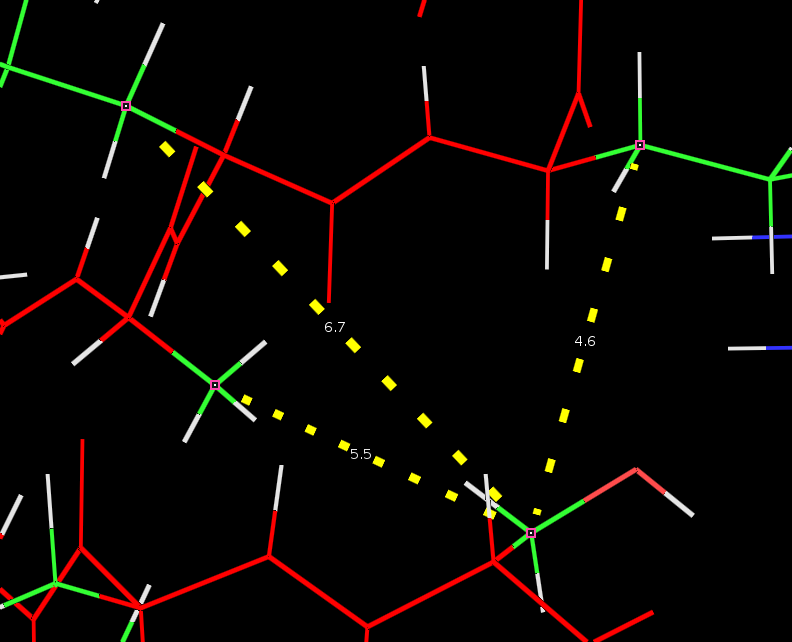
\includegraphics[width=0.5\textwidth]{img/constraints}
\end{frame}

\section{Grouping of constraints}
\frame{\tableofcontents[currentsection]}


\begin{frame}{grouping based on secondary structure}
    \centering
    \tiny
    \texttt{
MSALQPSRSYRITGYSPAISNGYRQRLFSMGLLPGAALRVVRIAPLGDPIQVETRQTSLALRRKDLALLTLVPLD\\
LLLLLLLSSSSSSSSLLLLLLLHHHHHHHHLLLLSSSSSSSSLLLLLLLSSSSLLLLSSSSLHHHHHHSSSSSLL\\}
    \normalsize
    \vspace{.5cm}
    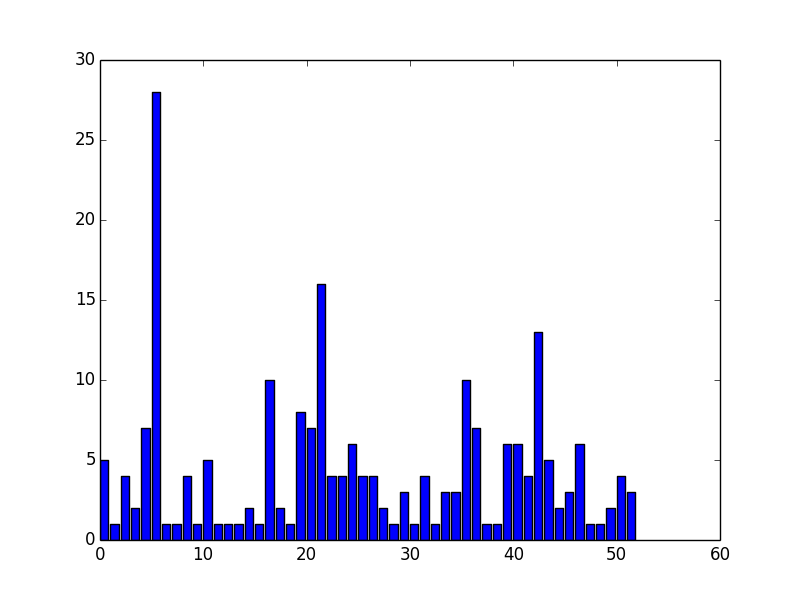
\includegraphics[width=0.8\textwidth]{img/contactMapGroupAmounts}
\end{frame}


\begin{frame}{grouping based on secondary structure}
    \centering
    \tiny
    \texttt{
MSALQPSRSYRITGYSPAISNGYRQRLFSMGLLPGAALRVVRIAPLGDPIQVETRQTSLALRRKDLALLTLVPLD\\
LLLLLLLSSSSSSSSLLLLLLLHHHHHHHHLLLLSSSSSSSSLLLLLLLSSSSLLLLSSSSLHHHHHHSSSSSLL\\}
    \normalsize
    \vspace{.5cm}
    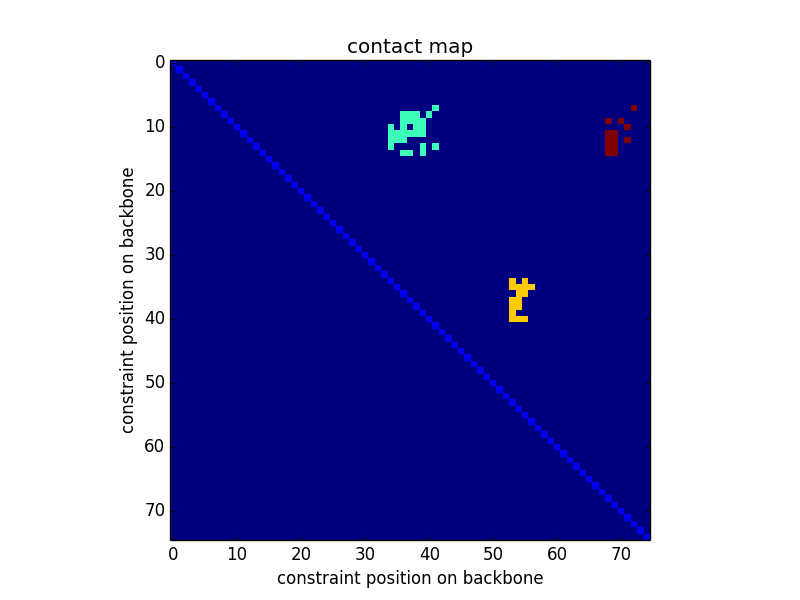
\includegraphics[trim = 25mm 0mm 25mm 10mm, clip, width=0.5\textwidth]{img/contactMapLargeGroups}
    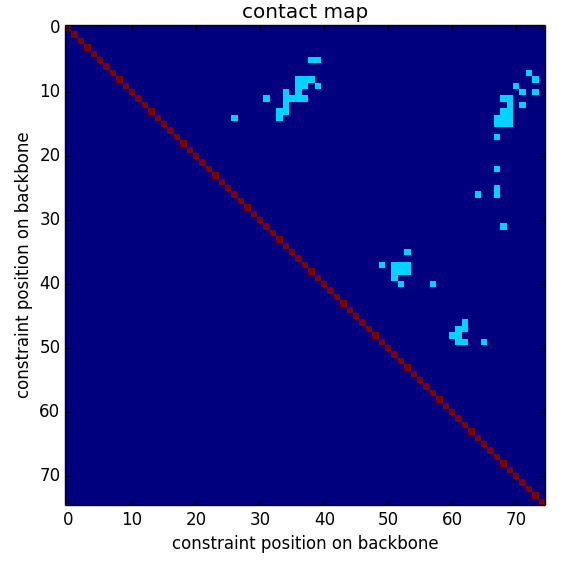
\includegraphics[width=0.5\textwidth]{img/contactMapNatives}
\end{frame}

\begin{frame}{Constraint visualisation in native}
    \centering
    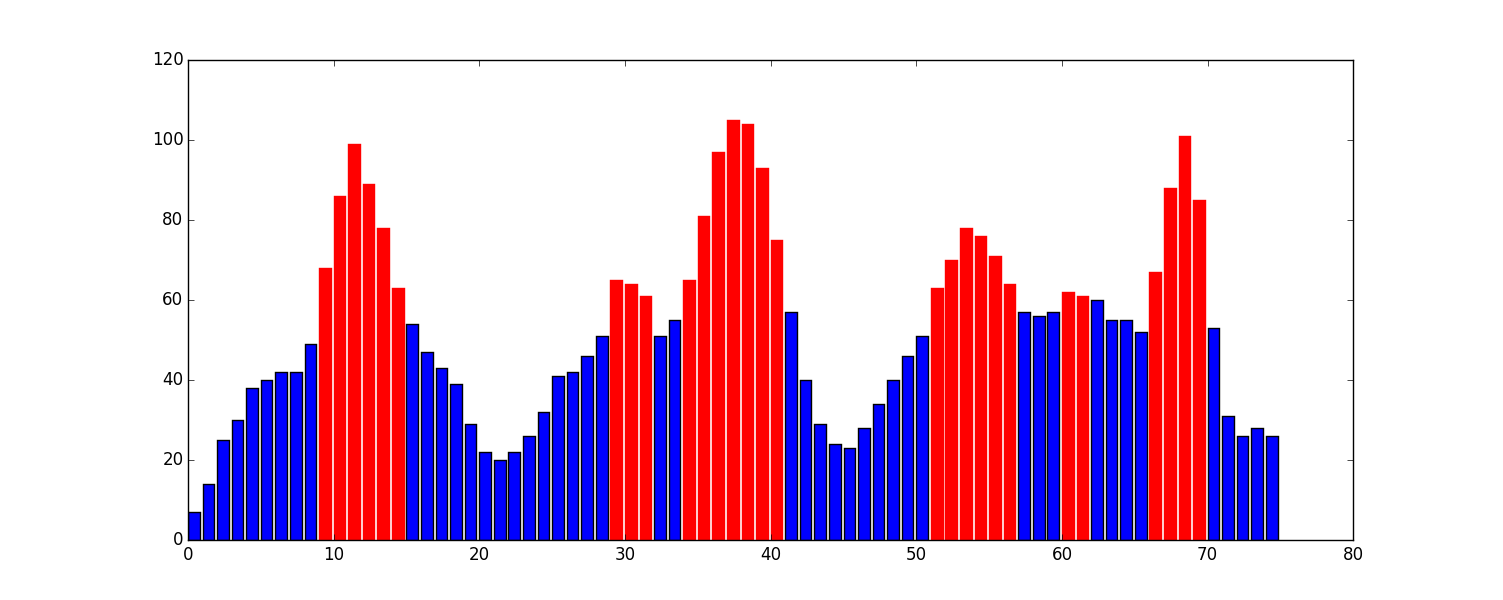
\includegraphics[width=\textwidth]{img/occurrenceBar}
\end{frame}


\begin{frame}{grouping based on occurrences}
    \centering
    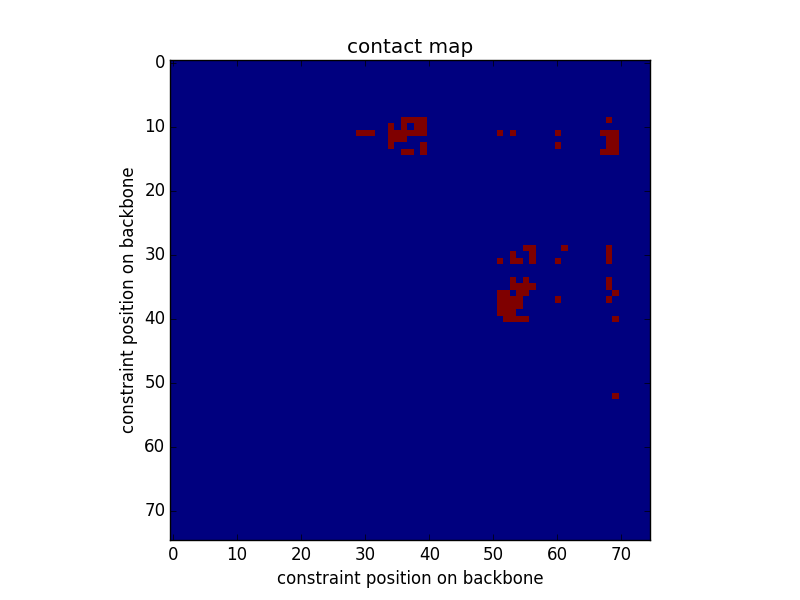
\includegraphics[trim = 25mm 0mm 25mm 10mm, clip,width=0.5\textwidth]{img/groupByOccurrence}
    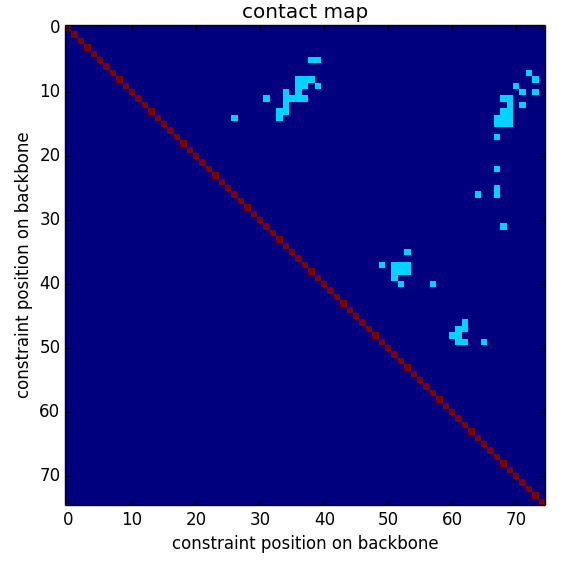
\includegraphics[width=0.5\textwidth]{img/contactMapNatives}
\end{frame}

\section{Planning}
\frame{\tableofcontents[currentsection]}
\begin{frame}{Project Timeline}
\begin{itemize}
%\item project runs for 8 weeks: 48 -- 3
%\item kickoff: 
%    \begin{itemize}
%    \item implement restraint grouping
%    \end{itemize}
\item milestone I: today (Week 50)
    \begin{itemize}
    \item introduce probability for constraints based on cluster membership
    \item Monte Carlo
        \begin{itemize}
        \item start value: clustering
        \item adopt probability based on rosetta score
        \item[$\Rightarrow$] different update mechanisms possible
        \end{itemize}
    \end{itemize}
\item milestone II: 9th January (Week 2)
    \begin{itemize}
    \item create poster, analyze results
    \end{itemize}
\item final poster session: 15th January (Week 3)
\end{itemize}
\end{frame}


% Since this a solution template for a generic talk, very little can
% be said about how it should be structured. However, the talk length
% of between 15min and 45min and the theme suggest that you stick to
% the following rules:  

% - Exactly two or three sections (other than the summary).
% - At *most* three subsections per section.
% - Talk about 30s to 2min per frame. So there should be between about
%   15 and 30 frames, all told.

\end{document}